\subsection*{jtr\_env\_v0}
Replicates Roman's reinforcement learning setup while following the gym interface.As can be seen from the the training reward graph below in Figure \ref{fig:jtr-v0}, there are no bounds for rewards. The rewards reach hundreds of thousands per episode, which makes judging the agent from rewards difficult. Plus the reward function Roman \cite{roman} used only gave rewards based on how close it is to the historical route. There are no rewards based on speed or time taken. It is clear that we need a better reward function.

\begin{figure}[h]
\centering
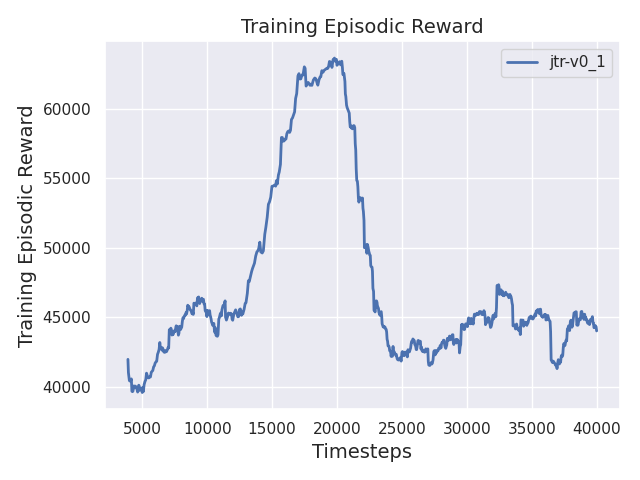
\includegraphics[width = 0.6\hsize]{figures/rl-refinements/jtr-v0.png}
\caption{jtr-v0 training reward graph with SAC}
\label{fig:jtr-v0}
\end{figure}

\subsection*{jtr\_env\_v1}
Reward function inspired from CarRacing-v0 \cite{CarRacing-v0} that is capped at 1000.
Reduced observation space with 6 features: 
\begin{itemize}
    \item Speed\_ov\_ground
    \item Heading\_ov\_ground\_cos, Heading\_ov\_ground\_sin,
    \item  Relative Latitude, Relative Longitude\_cos, Relative Longitude\_sin
\end{itemize}
The last 3 features are relative position between the current boat position and the goal position.

As can be seen in Figure \ref{fig:jtr-v1-training}, the training reward trend is downwards. The cause of this trend was explored in Section \ref{sec:state-estimator-problem} - \nameref{sec:state-estimator-problem}

\begin{figure}[h]
\centering
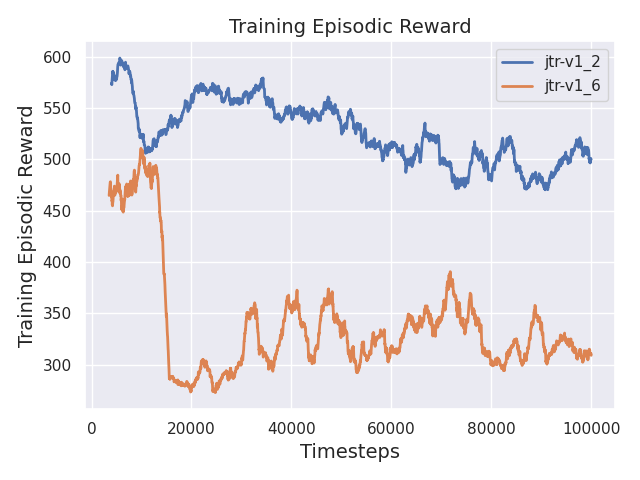
\includegraphics[width = 0.6\hsize]{figures/rl-reward-plots/jtr-v1 100k.png}
\caption{jtr-v1 training reward graph with SAC using Default(blue) vs gSDE(orange) hyperparameters}
\label{fig:jtr-v1-training}
\end{figure}

\subsection*{jtr\_env\_v1\_parallel}
jtr\_env\_v1 parallelized with Joblib using shared memory. Uses more resources but runs slower than jtr\_env\_v1, therefore jtr\_env\_v1 was used instead.

\subsection*{jtr\_env\_her\_v0}
Attempt to make use of Hindsight Experience Replay \cite{her-paper} which makes goal oriented environments more efficient. Implements the OpenAI GoalEnv class \cite{openai-gym}. It gives and error, and could not be run due to lack of documentation or examples of Hinsight Experince Replay functions and how they are called.

\subsection*{jtr\_env\_modelless\_v0}
First iteration of the modelless environments. Does not use any state estimator models. The speed is constant through the episode, and it is equal to the average of the previous 30 seconds, rounded up to the 4th decimal point. The heading is calculated directly from rudder, such that if the rudder is turned right 10 degrees, the heading will turn right 10 degrees in the next second.

Same observation space with jtr\_env\_v1.

-300 penalty for not reaching the goal, and reset the environment if taking too long to reach goal.

\subsection*{jtr\_env\_modelless\_v1}
Simplify the observation space to 4 features:
\begin{itemize}
    \item Speed\_ov\_ground
    \item Heading\_ov\_ground as angle,
    \item Relative Latitude and Longitude as angle
\end{itemize}

\subsection*{jtr\_env\_modelless\_v2}
Remove reward when moving away from the goal, add penalty for rudder angles. The penalty for rudder angles helped the agent to learn that the going straight is faster.

\subsection*{jtr\_env\_modelless\_v3}
First environment that can reach the goal consistently!

Inspired from existing autopilot systems, further simplify the observation space to 2 features:
\begin{itemize}
    \item Heading\_ov\_ground,
    \item Heading required to reach the goal at that timestep.
\end{itemize}
Speed was removed as it is constant through the episode. Latitude and Longitude were removed as those should not affect how the agent steers the boat.

\subsection*{jtr\_env\_modelless\_v4}
Remove rudder penalties as they are necessary to make the boat go faster in real life.

Update the reward function, reaching to goal reduced to 200 from 1000. Reward penalty for not reaching the goal at the end the episode changed to -50 from -300.

Finishing at the same time with the historical boat is 100. Solved is >100, which means the agent can reach the goal faster than historical boat.

Converges in less than 15 thousand step with both SAC and TQC algorithms. Can consistently reach the goal faster than the historical boat.

\section*{Further Details}
Further details and trained models can be found in the CONCI01-RL folder, which contains the trained models, training run details for each run and its own README file.